\section{Sistemas}

\begin{frame}{Sistemas}
    \begin{itemize}
        \item Un \textit{sistema} es un conjunto de elementos interdependientes que interactúan hacia el logro de un objetivo en común \cite{LK}.
        \item Durante el modelado, es necesario determinar los límites entre el sistema y su entorno. Esta decisión puede depender de los objetivos del estudio \cite{LK}.
        
    \end{itemize}
\end{frame}

\subsection{Componentes de un sistema}

\begin{frame}{Entidades}
    \begin{itemize}
        \item Una \textit{entidad} es un objeto de interés dentro del sistema.
        \item La mayoría de entidades representan objetos reales dentro del sistema. Sin embargo, en ocasiones se utilizan entidades \textit{dummies} o falsas para representar algunas situaciones dentro del sistema \cite{KSS}.
    \end{itemize}
\end{frame}

\begin{frame}{Atributos}
    \begin{itemize}
        \item Un \textit{atributo} es una propiedad de una entidad.
        \item Los atributos son características comunes para todas las entidades, pero cada entidad puede tener un valor diferente para cada característica.
    \end{itemize}
\end{frame}

\begin{frame}{Variables de estado}
    \begin{itemize}
        \item Una \textit{variable} representa un valor o característica de todo el sistema.

        \item Pueden ser escalares, vectores o matrices, suelen representar valores que cambian a lo largo de la simulación.
        
        \item Son accesibles por cualquier entidad, pertenecen al sistema y tienen un valor único en cada momento (ej: Reloj de la simulación).
    \end{itemize}
\end{frame}

\begin{frame}{Estado del sistema}
    \begin{itemize}
        \item El \textit{estado del sistema} se define como el conjunto mínimo de variables necesarias para caracterizar o describir todos aquellos aspectos de interés del sistema en un instante dado.
        
    \end{itemize}
\end{frame}

\begin{frame}{Recursos}
    \begin{itemize}
        \item Un \textit{recurso} se refiere a un servidor (operario, máquina, ubicación, etc.) capaz de ofrecer algún servicio a las entidades.
        \item Se asocia a restricciones del sistema.
        \item Las entidades compiten por el uso de los recursos. 
    \end{itemize}
\end{frame}

\begin{frame}{Actividades}
    \begin{itemize}
        \item Una \textit{actividad} representa un lapso de una duración especificada.
        \item Se asocia a menudo operaciones que demandan tiempo de uno o más recursos.
    \end{itemize}
    %------------------------
    %Incluir Listas y el Reloj
\end{frame}



\begin{frame}{Eventos}
    \begin{itemize}
        \item Un \textit{evento} se define como una ocurrencia instantánea que puede cambiar el estado del sistema.
        
        \item Durante la simulación se lleva un registro de los eventos que se espera que ocurran en el futuro; esta información se almacena en un \textit{calendario de eventos}.%\pause

    \end{itemize}
\end{frame}

\begin{frame}{Ejemplos}
\small{
\begin{table}[]
\begin{tabular}{|l|l|l|l|}
\hline
\textbf{Sistema}                                                       & Bancario                                                                                                & Producción                                                                                & Inventario                                                                     \\ \hline
\textbf{Entidad}                                                       & Cliente                                                                                                 & \begin{tabular}[c]{@{}l@{}}Órdenes de\\ producción\end{tabular}                           & Productos                                                                      \\ \hline
\textbf{Atributo}                                                      & \begin{tabular}[c]{@{}l@{}}Edad\\ Saldo en cuenta\end{tabular}                                          & \begin{tabular}[c]{@{}l@{}}Tamaño de orden\\ Prioridad del cliente\end{tabular}           & \begin{tabular}[c]{@{}l@{}}Volumen\\ Ubicación\end{tabular}                    \\ \hline
\textbf{Actividad}                                                     & Depósito                                                                                                & \begin{tabular}[c]{@{}l@{}}Soldadura\\ Maquinado\end{tabular}                             & \begin{tabular}[c]{@{}l@{}}Inspección\\ Picking\end{tabular}                   \\ \hline
\textbf{Evento}                                                        & \begin{tabular}[c]{@{}l@{}}Llegada\\ Salida\end{tabular}                                                & \begin{tabular}[c]{@{}l@{}}Falla de una \\ máquina\end{tabular}                           & \begin{tabular}[c]{@{}l@{}}Llegada de un\\ pedido\end{tabular}                 \\ \hline
\textbf{\begin{tabular}[c]{@{}l@{}}Variables\\ de estado\end{tabular}} & \begin{tabular}[c]{@{}l@{}}Número de \\ cajeros ocupados\\ Número de \\ clientes esperando\end{tabular} & \begin{tabular}[c]{@{}l@{}}Estado de \\ las máquinas\\ Producto en\\ proceso\end{tabular} & \begin{tabular}[c]{@{}l@{}}Nivel de inventario\\ Demanda atrasada\end{tabular} \\ \hline
\end{tabular}
\end{table}
}
\end{frame}

\subsection{Tipos de sistemas}

\begin{frame}{Tipos de sistemas}
\begin{columns}
\begin{column}{0.5\textwidth}
    Un sistema discreto es aquel en el cual las variables de estado cambian solo en puntos discretos en el tiempo.
\begin{figure}
    \centering
    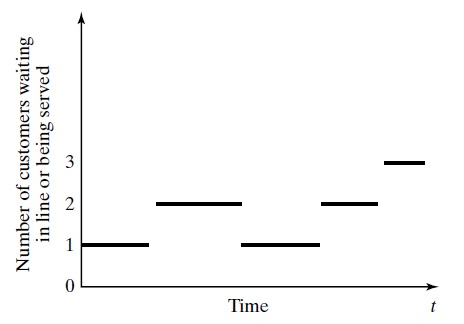
\includegraphics[width=4.5cm]{images/discreto.jpg}
    \caption{Sistema discreto}
    \label{fig:sistdiscreto}
\end{figure}
\end{column}
\begin{column}{0.5\textwidth} 
    Un sistema continuo es aquel en el cual las variables de estado cambian continuamente a lo largo del tiempo.
\begin{figure}
    \centering
    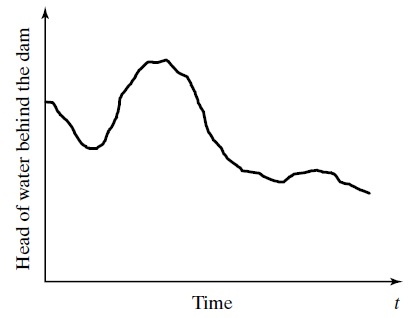
\includegraphics[width=4.5cm]{images/continuo.jpg}
    \caption{Sistema continuo}
    \label{fig:sistcontinuo}
\end{figure}
\end{column}
\end{columns}
\end{frame}



